% Created 2017-02-01 Wed 22:02
% Intended LaTeX compiler: pdflatex
\documentclass[presentation]{beamer}
\usepackage[utf8]{inputenc}
\usepackage[T1]{fontenc}
\usepackage{graphicx}
\usepackage{grffile}
\usepackage{longtable}
\usepackage{wrapfig}
\usepackage{rotating}
\usepackage[normalem]{ulem}
\usepackage{amsmath}
\usepackage{textcomp}
\usepackage{amssymb}
\usepackage{capt-of}
\usepackage{hyperref}
\usetheme{default}
\author{Will Rempel}
\date{\today}
\title{}
\hypersetup{
 pdfauthor={Will Rempel},
 pdftitle={},
 pdfkeywords={},
 pdfsubject={},
 pdfcreator={Emacs 25.0.50.1 (Org mode 9.0.3)}, 
 pdflang={English}}
\begin{document}

\begin{frame}{Outline}
\tableofcontents
\end{frame}

\section{Theoretical Background}
\label{sec:orgeb84d66}
\subsection{Overview}
\label{sec:org9345558}
\begin{itemize}
\item Feed-forward, supervised learning
\item Uses backpropagation algorithms
\item coNN - constructive neural network
\begin{itemize}
\item 2 main categories:
\begin{itemize}
\item evolutionary based (what is done at Brock)
\item generally constructive. CCNN is main exemplar of this group
\end{itemize}
\end{itemize}
\end{itemize}
\subsection{Overview II}
\label{sec:orgb89dcee}
\begin{itemize}
\item creates it's own topology starting with minimal network
\begin{itemize}
\item input and output layers only, as usual connected by weights.
\end{itemize}
\item input of nodes code the problem being presented to the network
\item output of nodes code the network's response to the input problem
\item typically quickprop is used as the learning rule
\end{itemize}
\subsection{Basic Algorithm}
\label{sec:org9411f56}
\begin{frame}[label={sec:org2b7dbb6}]{Step 1 Training input weights}
  A new hidden neuron is added one at a time
  Instead of a minimum, we find a maximum: the maximum correlation between the candidate output and the residual error of the networks output.

  \begin{enumerate}
  \item generate a population of candidate nodes with randomized input weights
  \item inputs are connected, but not outputs
  \item repeat training steps until no correlation improvement
  \begin{enumerate}
  \item one epoch of the training data is run through
  \item update input weights using any learning rule, such that correlation is increased
  \end{enumerate}
  \end{enumerate}
\end{frame}


\begin{frame}
  \frametitle{Train input weights - correlation}
	\begin{columns}[t]
		\begin{column}[t]{0.5\textwidth}
      \small{S is sum over all output units $\mathit{o}$ of correlation with error}
      $$ S = \sum_{o} \lvert \sum_{p} (V_{p} - V) (E_{p,o} - E_{o}) \rvert $$
     \\  
      \begin{center}
        \begin{tabular}{ll}
          \(\mathit{o}\) & \tiny{network output at which the error is measured} \\
          p & \tiny{the training pattern} \\
          \(\sigma\) & \tiny{network output} \\
          V\(_{\text{p}}\) & \tiny{candidate output for input pattern p}   \\
          E\(_{\text{p,o}}\) & \tiny{network output error for output o, pattern p} \\
          \(\overline{V}\) & \tiny{average of candidate output over all patterns} \\
          \(\overline{E_{o}}\) & \tiny{average of output errors over all patterns} \\
        \end{tabular}
      \end{center}
		\end{column}
		\begin{column}{0.5\textwidth}
      \begin{figure}
        \centering
        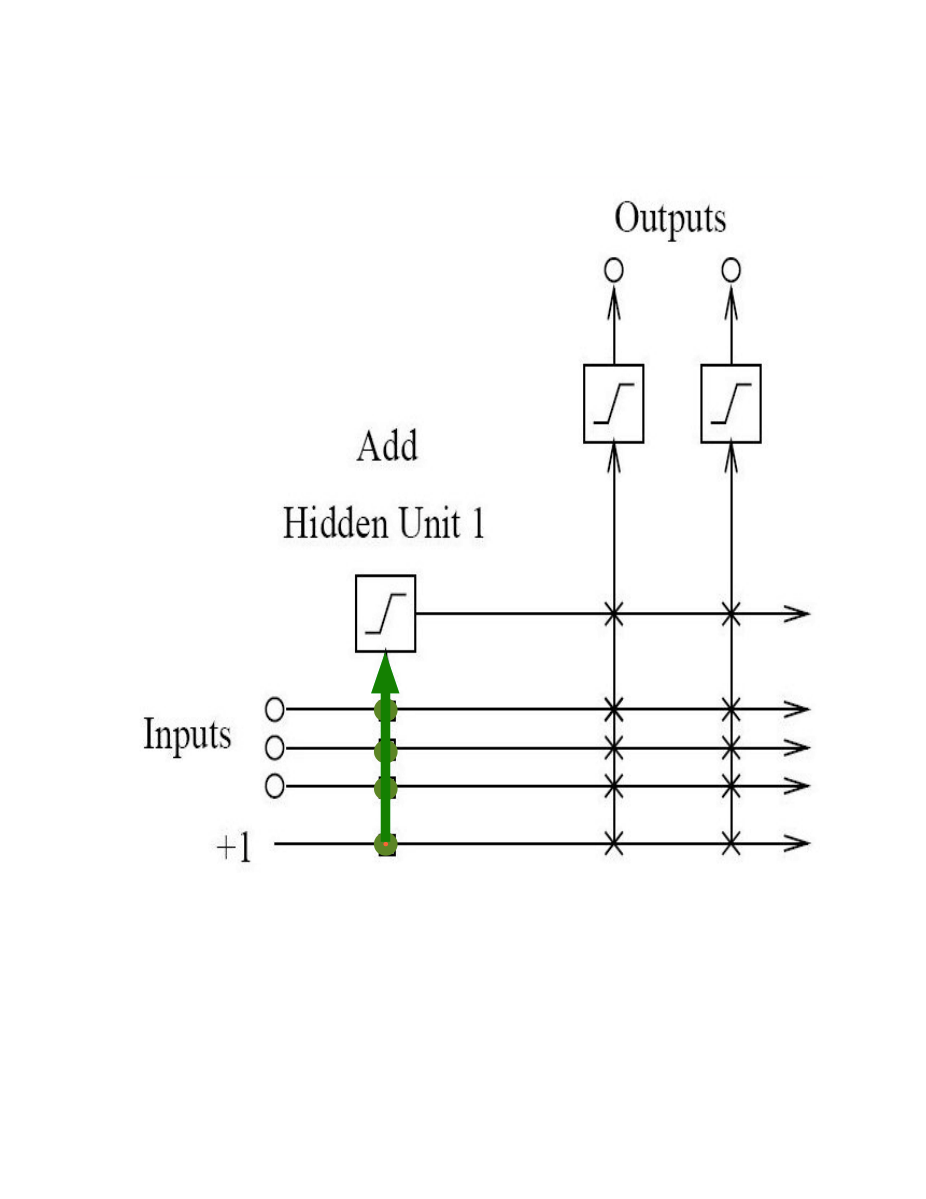
\includegraphics[scale=0.28]{trainInputunit.png}
        \caption{image}
      \end{figure}			
		\end{column}
	\end{columns}
\end{frame}


\begin{frame}
  \frametitle{Train input weights - correlation}
	\begin{columns}[t]
		\begin{column}{0.5\textwidth}
      $$ \frac{\delta S}{\delta w_{i}} = \sum_{p,o} \sigma_{o}(E_{p,o} - \overline{E_{o}}) \mathit{f_{p}}^{\prime} I_{i,p} $$
     \\ 
      \begin{center}
        \begin{tabular}{ll}
          \(\mathit{w_{i}}\) & \tiny{weight to be updated}  \\
          \(\sigma_{o}\) & \tiny{sign of correlation}  \\
          \(\mathit{f_{p}}^{\prime}\) & \tiny{derivative for pattern p of the nodes fn wrt of inputs} \\
          I\(_{\text{i,p}}\) & \tiny{input node gets from unit i for input p}  \\
          E\(_{\text{p,o}}\) & \tiny{network output error for output o, pattern p} \\
          \(\overline{E_{o}}\) & \tiny{average of output errors over all patterns} \\
          & \\
        \end{tabular}
      \end{center}
		\end{column}
		\begin{column}{0.5\textwidth}
      \begin{figure}
        \centering
        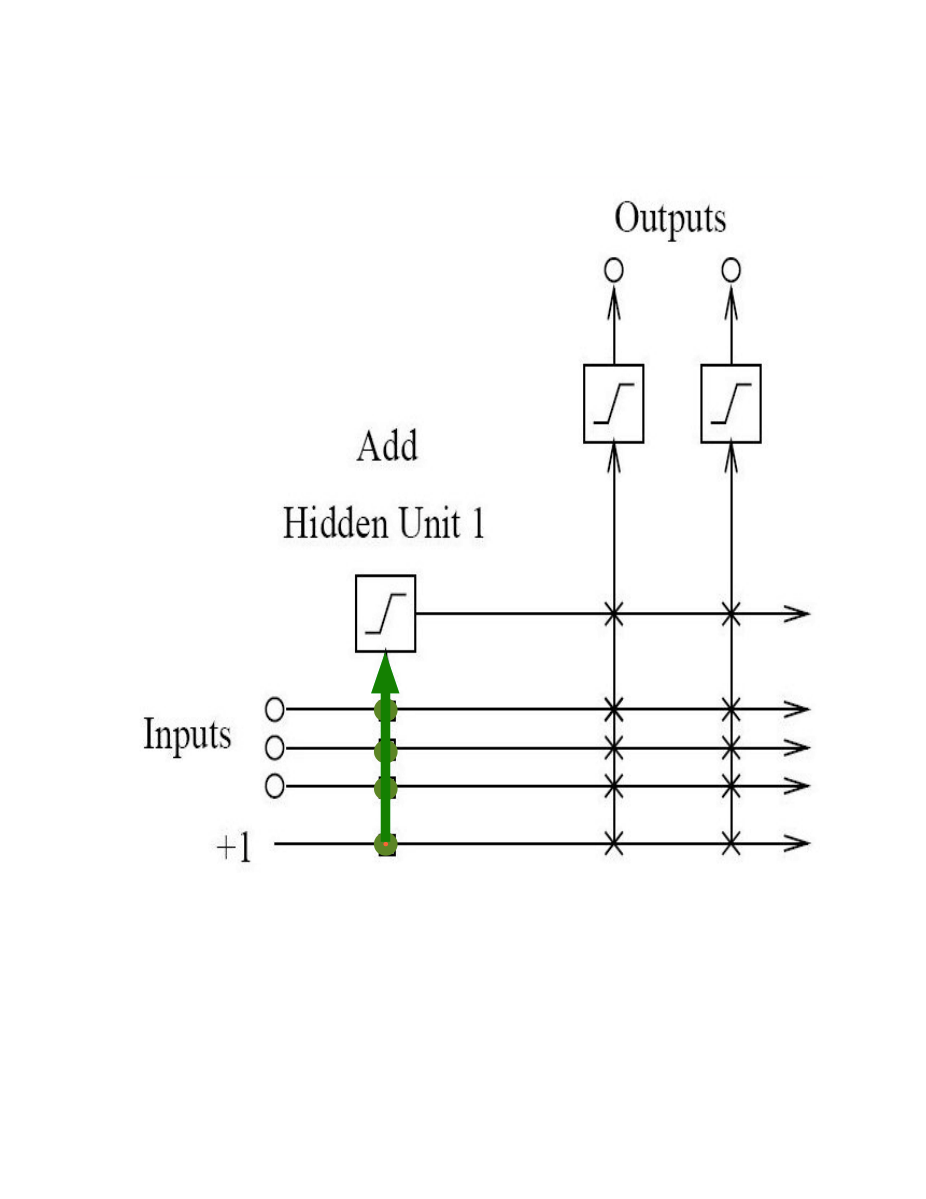
\includegraphics[scale=0.28]{trainInputunit.png}
        \caption{image}
      \end{figure}			
		\end{column}
	\end{columns}
\end{frame}



\begin{frame}{Step 1 Training input weights}
  \begin{itemize}
    \item candidate with highest correlation is put in the network, others are discarded.
    \item correlation sign doesn't matter, only magnitude
    \item the bias unit effectively implements a learnable resting activation level for each hidden and output unit.
    \item subsequent hidden neurons are attached to previous hidden neurons - this is where the cascade term comes from.
  \end{itemize}
\end{frame}

\begin{frame}[label={sec:org085d5cb}]{Step 2 Training output weights}
\begin{enumerate}
\item connect output of new node to output layer nodes
use randomized weights that have adjusted sign to reduce error
\item input weights are fixed
\item only output weights are trained using any learning rule, until no improvement in error reduction

\item once done the new node is fixed permanently.
\item any new training involves adding another new node on it's own downstream layer
\end{enumerate}
\begin{center}
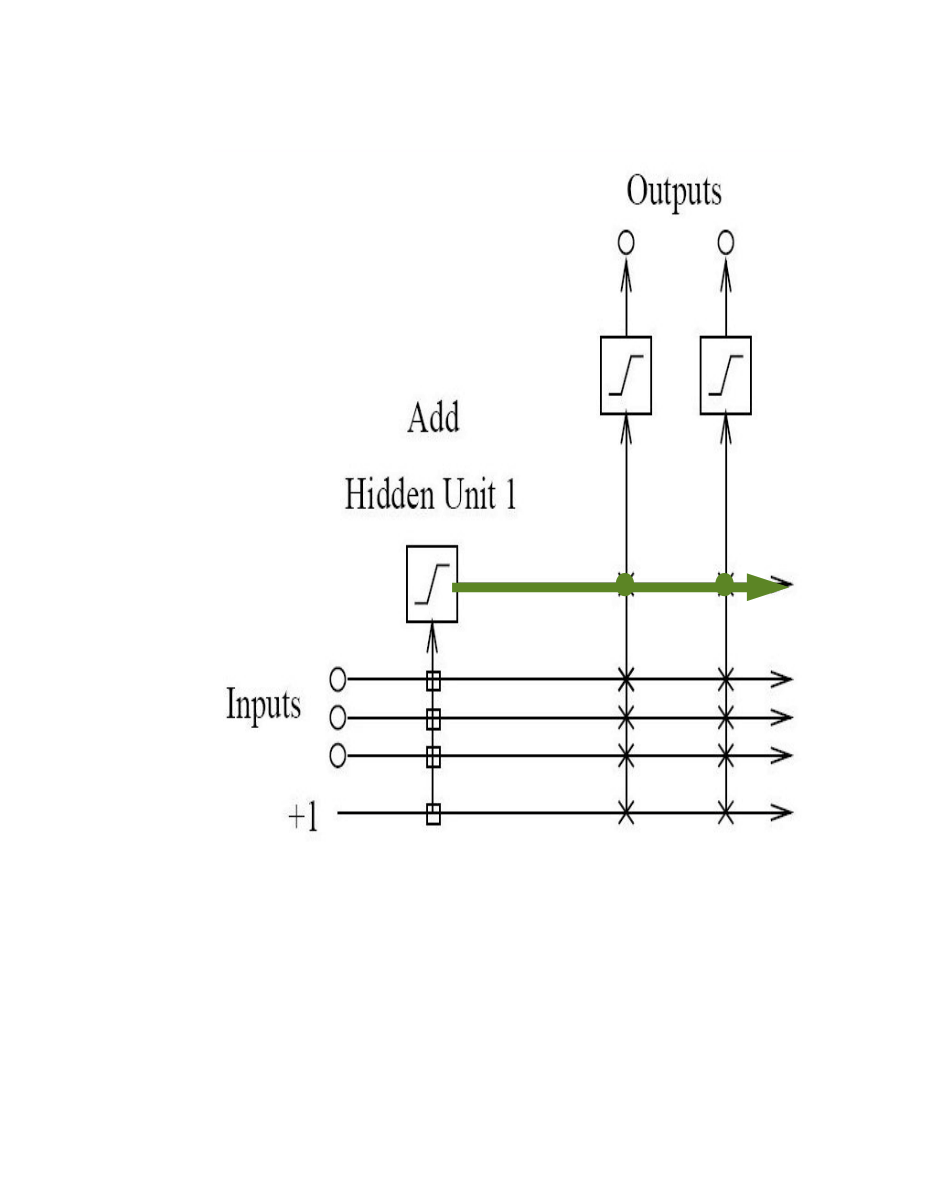
\includegraphics[scale=0.20]{trainoutputunit.png}
\end{center}
\end{frame}

\section{Comparisons}
\label{sec:org8f2bd35}
\subsection{Two Problems with Backpropagation}
\label{sec:org168fc30}
\begin{frame}[label={sec:org200ccae}]{The Step Size Problem}
\begin{itemize}
\item vanilla backpropagation requires small steps for convergence - slow
\item we do not have the information to pick an optimal learning rate, manually selected
\end{itemize}
\end{frame}
\begin{frame}[label={sec:orgde08e3c}]{The Moving Target Problem}
\begin{itemize}
\item complication when many factors changing at the same time
\item error signal defines problem unit trying to solve, but this keeps changing
\item dramatic slowdown of training with increasing number of hidden layers
\item herd effect:
\begin{itemize}
\item 2 tasks A, B. If A has bigger effect, all nodes redundantly train for A, ignoring B
\item But when all nodes move toward B at once, problem A response becomes worse.
\item eventually nodes split to train for separate problems A and B, but it takes a long time
\item a randomly initialized network prevents nodes from behaving identically, but this tends to dissipate as the network is trained
\end{itemize}
\item One way to combat: allow only a few weights to change while keeping the others constant
\end{itemize}
\end{frame}
\subsection{Pros \& Cons}
\label{sec:orgca4894d}
\frame{
\frametitle{Pros}
\begin{itemize}
\item At elast 10 times faster than standard backpropagation
\begin{itemize}
\item\relax [performanceChart2.png]
\end{itemize}
\item The network determines its own size and topologies
\item Incremental/life long learning: new training, new information can be added, with an already trained network
\item effectively deals with the step size and moving target problems
\end{itemize}
}
\frame{
  \frametitle{Cons}
\begin{itemize}
\item Very susceptible to overfitting
\end{itemize}
}

\section{Applications}
\label{sec:orgea347f6}
\label{sec:orgc59e772}
\frame{
  \frametitle{Applications}

In spite of the many CoNN algorithms surveyed in (Kwok \& Yeung, 1997a), the most popular for regression problems is no doubt the Cascade Correlation algorithm and maybe the second most popular is the DNC\ldots{}
The popularity of Cascade Correlation can be attested by the various ways this
algorithm has inspired new variations and also has been used in the combined
approaches between learning methods. [Franco et al, 2009] 

}


\begin{frame}[allowframebreaks, t]{References}
  \tiny
  \begin{thebibliography}{99}
    \bibitem[]{} S. E. Fahlman and C. Lebiere, “The cascade-correlation learning 
    architecture.” \\
    \bibitem{} K. Khatter and J. Kaur, “Global Journal of Engineering Science and
    Research Management.” \\
    \bibitem{} S. K. Sharma and P. Chandra, “CONSTRUCTIVE NEURAL NETWORKS: A REVIEW,”
    International Journal of Engineering Science and Technology, vol. 1, no. 2,
    pp. 7847–7855. \\
    \bibitem{} T.-Y. Kwok and D.-Y. Yeung, “Constructive algorithms for structure
    learning in feedforward neural networks for regression problems,” IEEE
    Transactions on Neural Networks, vol. 8, no. 3, pp. 630–645, 1997. \\
    \bibitem{} G. Balázs, “Cascade-Correlation Neural Networks: A Survey.” \\
    \bibitem{} Y. Guo, L. Bai, S. Lao, S. Wu, and M. S. Lew, “A Comparison between
    Artificial Neural Network and Cascade-Correlation Neural Network in Concept
    Classification,” in Advances in Multimedia Information Processing – PCM
    2014, 2014, pp. 248–253. \\ 
    \bibitem{} B. K. Wong, T. A. Bodnovich, and V. S.-K. Lai, “The Use of
    Cascade-Correlation Neural Networks in University Fund Raising,” The Journal
    of the Operational Research Society, vol. 51, no. 8, pp. 913–920, 2000. \\
    \bibitem{} A. B. Nassif, L. F. Capretz, and D. Ho, “Software Effort Estimation in
    the Early Stages of the Software Life Cycle Using a Cascade Correlation
    Neural Network Model,” in 2012 13th ACIS International Conference on
    Software Engineering, Artificial Intelligence, Networking and
    Parallel/Distributed Computing, 2012, pp. 589–594. \\
    \bibitem{} S. Saha, A. Konar, A. Saha, A. K. Sadhu, B. Banerjee, and A. K. Nagar,
    “EEG based gesture mimicking by an artificial limb using cascade-correlation
    learning architecture,” in 2016 International Joint Conference on Neural
    Networks (IJCNN), 2016, pp. 4680–4687. \\
    \bibitem{} P. Blonda, G. Pasquariello, and J. Smid, “Comparison of backpropagation,
    cascade-correlation and Kokonen algorithms for cloud retrieval,” in
    Proceedings of 1993 International Conference on Neural Networks
    (IJCNN-93-Nagoya, Japan), 1993, vol. 2, pp. 1231–1234 vol.2. \\
    \bibitem{} N. Sharma and H. Om, “Cascade correlation neural network model for
    classification of oral cancer,” WSEAS Transactions on Biology and
    Biomedicine, vol. 11, pp. 45–51, 2014. \\
    \bibitem{} B. Chandra and P. P. Varghese, “Applications of Cascade Correlation
    Neural Networks for Cipher System Identification,” World Academy of Science,
    Engineering and Technology, International Journal of Computer, Electrical,
    Automation, Control and Information Engineering, vol. 1, no. 2, pp. 369–372,
    2007. \\
    \bibitem{} N. A. Singh and T. Naryanan, “Application of Cascaded Correlation Neural
    Network for Financial Performance Prediction and Analysis of BSNL,” in
    Swarm, Evolutionary, and Memetic Computing, 2014, pp. 502–513. \\

    \end{thebibliography}
  \end{frame}

\end{document}